\documentclass[12pt,a4paper]{article}
\usepackage{amsmath,amscd,amsbsy,amssymb,latexsym,url,bm,amsthm}
\usepackage{epsfig,graphicx,subfigure}
\usepackage{enumitem,balance}
\usepackage{wrapfig}
\usepackage{mathrsfs,euscript}
\usepackage[usenames]{xcolor}
\usepackage{hyperref}
\usepackage[vlined,ruled,linesnumbered]{algorithm2e}
\usepackage{array}
\usepackage{float}
\hypersetup{colorlinks=true,linkcolor=black}

\newtheorem{theorem}{Theorem}
\newtheorem{lemma}[theorem]{Lemma}
\newtheorem{proposition}[theorem]{Proposition}
\newtheorem{corollary}[theorem]{Corollary}
\newtheorem{exercise}{Exercise}
\newtheorem*{solution}{Solution}
\newtheorem{definition}{Definition}
\theoremstyle{definition}

\renewcommand{\thefootnote}{\fnsymbol{footnote}}

\newcommand{\postscript}[2]
{\setlength{\epsfxsize}{#2\hsize}
	\centerline{\epsfbox{#1}}}

\renewcommand{\baselinestretch}{1.0}

\setlength{\oddsidemargin}{-0.365in}
\setlength{\evensidemargin}{-0.365in}
\setlength{\topmargin}{-0.3in}
\setlength{\headheight}{0in}
\setlength{\headsep}{0in}
\setlength{\textheight}{10.1in}
\setlength{\textwidth}{7in}
\makeatletter \renewenvironment{proof}[1][Proof] {\par\pushQED{\qed}\normalfont\topsep6\p@\@plus6\p@\relax\trivlist\item[\hskip\labelsep\bfseries#1\@addpunct{.}]\ignorespaces}{\popQED\endtrivlist\@endpefalse} \makeatother
\makeatletter
\renewenvironment{solution}[1][Solution] {\par\pushQED{\qed}\normalfont\topsep6\p@\@plus6\p@\relax\trivlist\item[\hskip\labelsep\bfseries#1\@addpunct{.}]\ignorespaces}{\popQED\endtrivlist\@endpefalse} \makeatother

\begin{document}
	\noindent
	
	%========================================================================
	\noindent\framebox[\linewidth]{\shortstack[c]{
			\Large{\textbf{Lab05-DynamicProgramming}}\vspace{1mm}\\
			CS214-Algorithm and Complexity, Xiaofeng Gao, Spring 2021.}}
	\begin{center}
		\footnotesize{\color{red}$*$ If there is any problem, please contact TA Haolin Zhou.}
		
		% Please write down your name, student id and email.
		\footnotesize{\color{blue}$*$ Name:Beichen Yu  \quad Student ID:519030910245 \quad Email: polarisybc@sjtu.edu.cn}
		
	\end{center}
	
	\begin{enumerate}
		\item \textit{Optimal Binary Search Tree.} Given a sorted sequence $K=\left \langle k_{1}, k_{2}, \ldots, k_{n} \right \rangle$ of $n$ distinct keys, and we wish to build a binary search tree from these keys. For each key $k_{i}$, we have a probability $p_{i}$ that a search will be for $k_{i}$. Some searches may be for values not in $K,$ and so we also have $n+1$ \emph{dummy keys} $d_{0}, d_{1}, d_{2}, \ldots, d_{n}$ representing values not in $K$. In particular, $d_{0}$ represents all values less than $k_{1}$, and $d_{n}$ represents all values greater than $k_{n}$. For $i=1,2, \ldots, n-1,$ the dummy key $d_{i}$ represents all values between $k_{i}$ and $k_{i+1}$. For each dummy key $d_{i}$, we have a probability $q_{i}$ that a search will correspond to $d_{i}$. Each key $k_{i}$ is an internal node, and each dummy key $d_{i}$ is a leaf. Every search is either successful (finding some key $k_{i}$ ) or unsuccessful (finding some dummy key $d_{i}$ ), and so we have $ \sum_{i=1}^{n} p_{i}+\sum_{i=0}^{n} q_{i}=1 $. 
		\begin{enumerate}
			\item Prove that if an optimal binary search tree $T$ ($ T $ has the smallest expected search cost) has a subtree $T^{\prime}$ containing keys $k_{i}, \ldots, k_{j},$ then this subtree $T^{\prime}$ must be optimal as well for the subproblem with keys $k_{i}, \ldots, k_{j}$ and dummy keys $d_{i-1}, \ldots, d_{j}$. 
			\item We define $e[i, j]$ as the expected cost of searching an optimal binary search tree containing the keys $k_{i}, \ldots, k_{j} .$ Our goal is to compute $e[1, n]$. Write the state transition equation and pseudocode using \textbf{dynamic programming} to find
			the minimum expected cost of a search in a given binary tree. (\textbf{Remark}: You may use $ w(i, j)=\sum_{l=i}^{j} p_{l}+\sum_{l=i-1}^{j} q_{l} $).
			\item Implement your proposed algorithm in C/C++ and analyze the time complexity. ({\color{blue}The framework Code-OBST.cpp is attached on the course webpage}). Give the minimum search cost calculated by your algorithm. The test case is given as following:
			\begin{table}[H]
				\setlength{\abovecaptionskip}{0cm}
				\setlength{\belowcaptionskip}{0.1cm}
				\centering		
				\begin{tabular}{|c|cccccccc|}
					\hline
					$ i $&0&1&2&3&4&5&6&7\\
					\hline
					$ p_{i} $&&0.04&0.06&0.08&0.02&0.10&0.12&0.14\\
					\hline
					$ q_{i} $&0.06&0.06&0.06&0.06&0.05&0.05&0.05&0.05\\
					\hline
				\end{tabular}
			\end{table}
			\item Please draw the structure of the optimal binary search tree in the test case, and explain the drawing process.   
		\end{enumerate}
		    \begin{solution}
		        \begin{enumerate}
		        \item If there is a subtree $T^{\prime \prime}$ has a smaller expected search cost than $T^{\prime}$. Then we can delete $T^{\prime}$ from $T$, and using $T^{\prime \prime}$ to substitute. Then we get a new binary search tree, which has a smaller expected search cost than $T$. So we got the contradiction, which means $T^{\prime}$ is the optimum solution.
		        \item If $j < i-1$, there is nothing the subtree. 
		        
		        If $j = i-1$, there is only a dummy key $d_{i-1}$ inside the subtree.  
		        
		        If $j > i-1$, we can find the root node $k_r$ of the subtree with nodes $k_i, k_{i+1}, \cdots, k_{j-1}, k_{j}$. The cost of the left subtree of $k_r$ is $e[i,r-1]$, and the cost of its right subtree is $e[r+1,j]$. If we link a subtree contains $k_i, k_{i+1}, \cdots, k_{j}$ to a root node, the depth of each node in the subtree adds 1, which means the total cost adds $w(i,j)=\sum_{l=i}^{j} p_{l}+\sum_{l=i-1}^{j} q_{l} $. So we have $e[i,j] = p_r + (e[i,r-1]+w(i,r-1)) + (e[r+1,j]+w(r+1,j))$. Because $w(i,r-1) + p_r +w(r+1,j) = w(i,j)$, we can conclude that $e[i,j] = e[i,r-1] + e[r+1,j] + w(i,j)$.\\
		        
		        So the state transition equation is:
		        
		        $$ e[i,j]=\left\{
				\begin{aligned}
					&q_{i-1}, & j = i-1; \\
					&\min_{i\leqslant r \leqslant j} \{e[i,r-1] + e[r+1,j] + w(i,j)\}, &i \leqslant j.
				\end{aligned}
				\right.
				$$
				
				To reduce complexity, we can use $w[i,j]$ to store the value of $w(i,j)$. When $j \geqslant i$ we have $w[i,j] = w[i,j-1] + p_j + q_j$.
				
				Next we propose our algorithm for optimal binary search tree:
				
				
				\begin{minipage}[t]{0.8\textwidth}
        \begin{algorithm}[H]
            \BlankLine
            \caption{Optimal-BST}
            Initialize two-dimensional arrays $e,w$ and $root$;

            \For{$i = 1$ \textbf{to} $n+1$} {
                $e[i][i-1] \leftarrow q_{i-1}$;\\
                $w[i][i-1] \leftarrow q_{i-1}$;
            }
            \For{$l = 1$ \textbf{to} $n$} {
            	\For{$i = 1$ \textbf{to} $n-l+1$} {
            		$j \leftarrow i+l-1$;\\
            		$e[i][j] \leftarrow \infty$;\\
            		$w[i][j] \leftarrow w[i][j-1] + p_j + q_j$;\\
            		\For{$r = 1$ \textbf{to} $j$} {
            			$t \leftarrow  e[i,r-1] + e[r+1,j] + w[i,j]$;\\
            			\If {$t < e[i][j]$}
            			{
            				$e[i][j] \leftarrow t$;\\
            				$root[i][j] \leftarrow r$;
            			}
            		}
            	}
            }
            \Return{$e$,$root$};
        \end{algorithm}
        \end{minipage}
				
				\item The code is included in the .zip file. 
				
				In the first for-loop, the time complexity is $O(n)$. In the second one, there are there for-loops inside. The time complexity is $O(1^2+2^2+\cdots + n^2) = O(n^3)$. So the total time complexity is $O(n^3)$.\\
				
				This is the result:
		       		\begin{figure}[H]
    \centering
    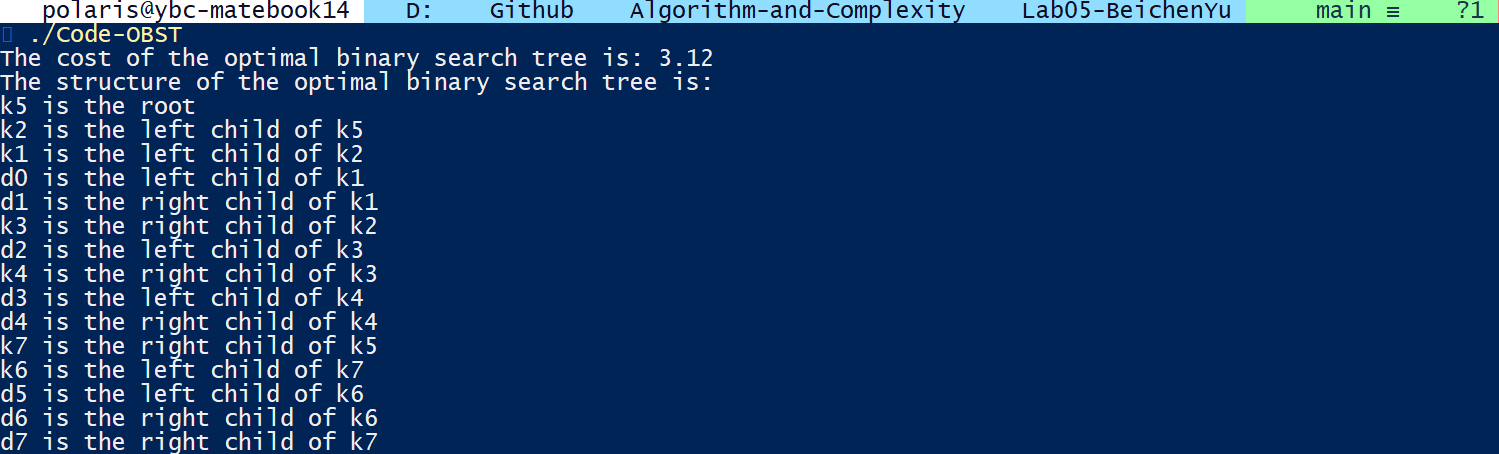
\includegraphics[width=0.8\textwidth]{obst.png}
    \caption{The result of the OBST}
\end{figure}
				\item I draw this  optimal binary search tree with powerpoint. The procress of drawing it is easy, just according to the output of the program and draw from the root to leaves.
				
				\begin{figure}[H]
    \centering
    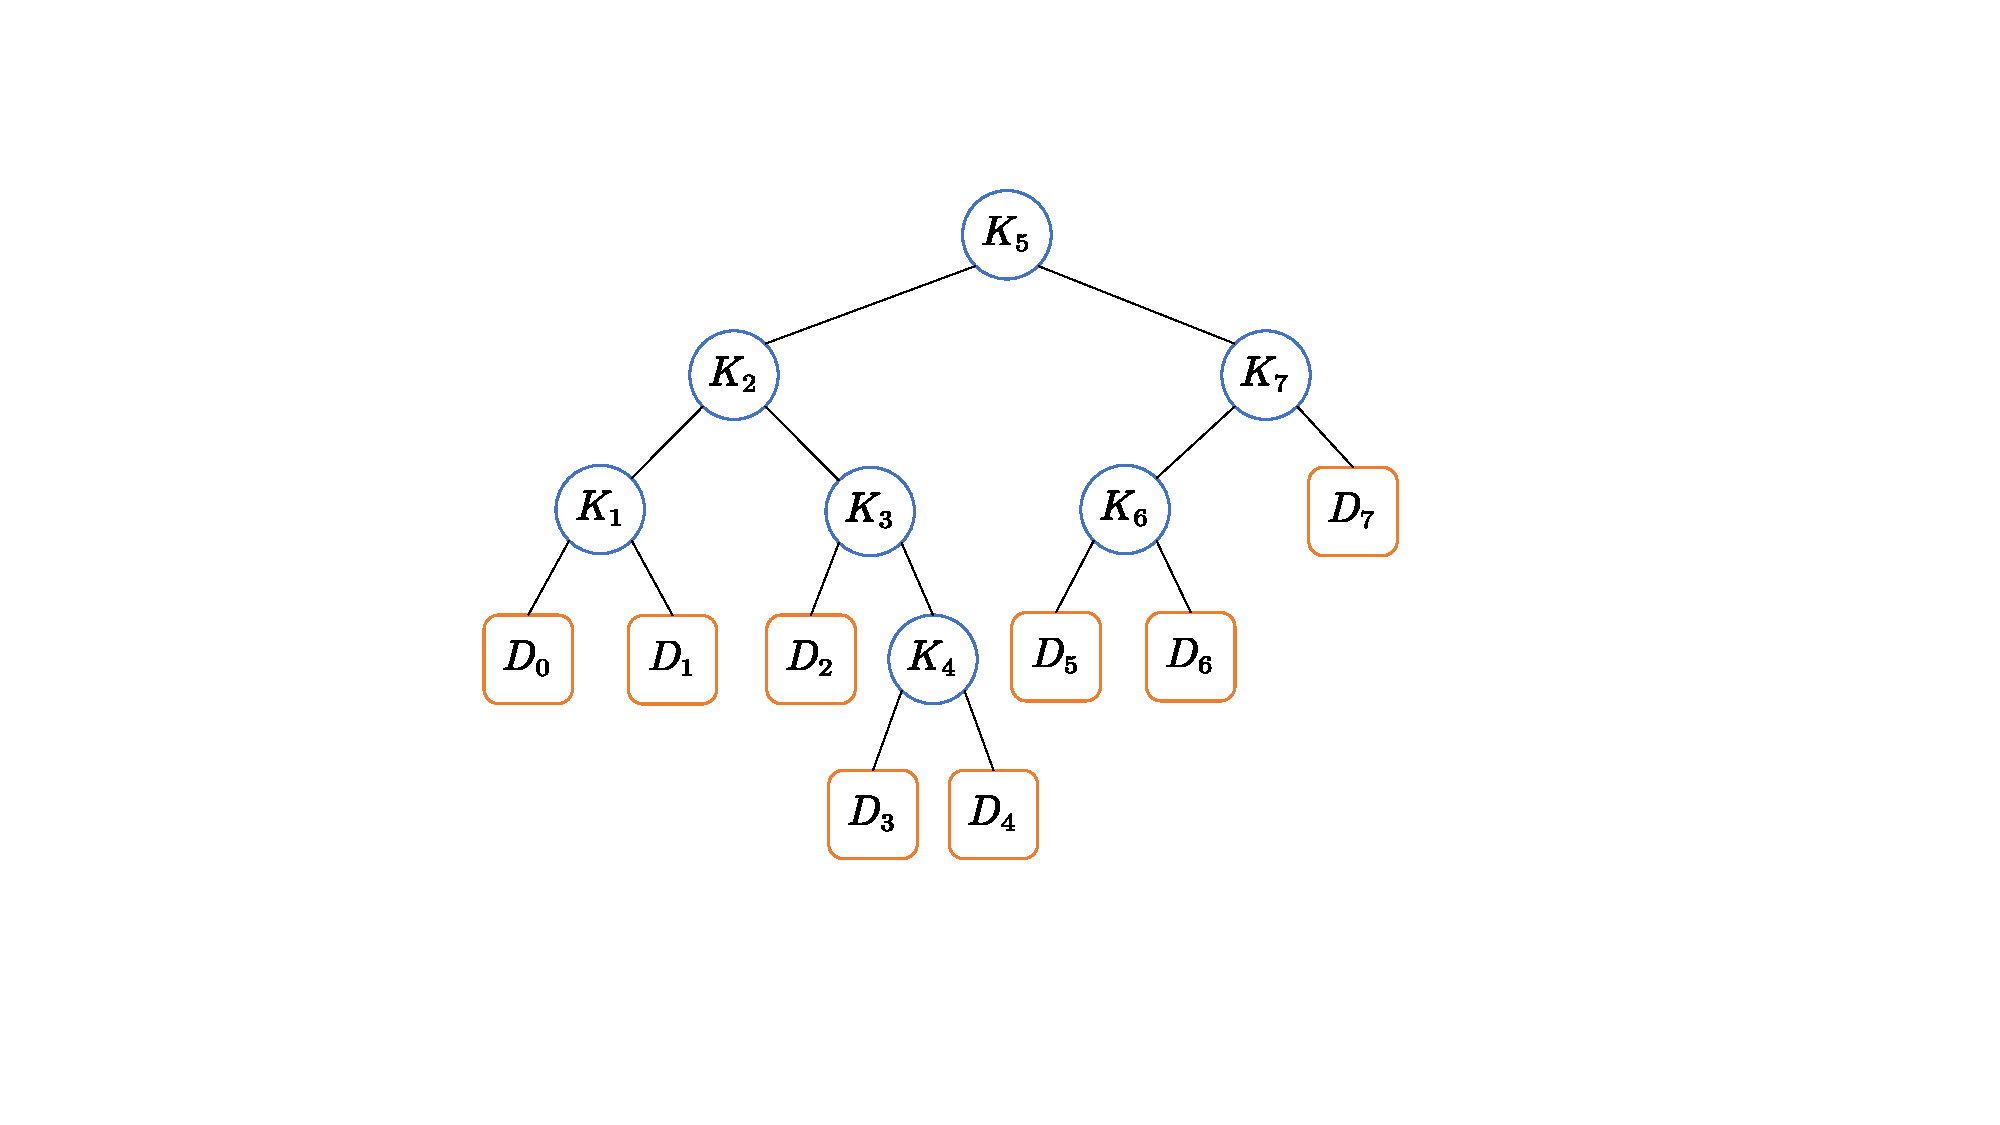
\includegraphics[width=0.5\textwidth]{opbst.pdf}
    \caption{The optimal binary search tree}
\end{figure}
		        \end{enumerate}
		    \end{solution}
		
		\item \textit{Dynamic Time Warping Distance.} \textbf{DTW} stretches the series along the time axis in a dynamic way over different
		portions to enable more effective matching. Let $D T W(i, j)$ be the optimal distance between the first $i$ and first $j$ elements of two time series $\bar{X}=\left(x_{1} \ldots x_{n}\right)$ and $\bar{Y}=\left(y_{1} \ldots y_{m}\right),$ respectively. Note that the two time series are of lengths $n$ and $m$, which may not be the same. Then, the value of $D T W(i, j)$ is defined recursively as follows:
		$$
		DTW(i, j)=\left|x_{i}- y_{j}\right|+\min(DTW(i, j-1), DTW(i-1, j), DTW(i-1, j-1))
		$$
		
		\begin{enumerate}
			\item Implement the proposed DTW algorithm in C/C++ and analyze the time complexity of your implementation. ({\color{blue}The framework Code-DTW.cpp is attached on the course webpage}). Two test cases have been given in the source code. 
			\item The window constraint imposes a minimum level $w$ of positional alignment between matched elements. The window constraint requires that $DTW(i, j)$ be computed only when $|i-j| \leq w$. Modify your code to add a window constraint and give the results of $ w=0 $ and $ w=1 $ on the two test cases. 
		\end{enumerate}
		    \begin{solution}
		       \begin{enumerate}
		       		\item The code is included in the .zip file. In the first several loops, there are only one for-loop, so the time complexity of these parts is $O(max\{m,n\})$. And in the biggest while-loop, there are $i = n - 1$ and $j = m-1$. Each time $i$ or $j$ or both of them minus one, so in this part the time complexity is $O(mn)$. So the finial time complexity is $O(mn)$.\\
		       		
		       		This is the result:
		       		\begin{figure}[H]
    \centering
    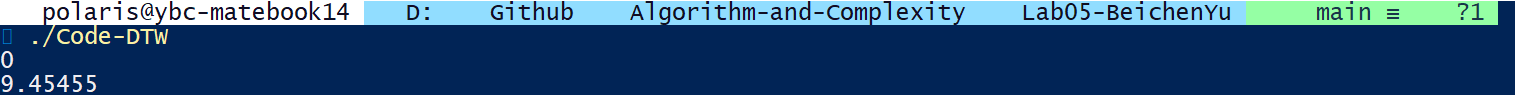
\includegraphics[width=0.8\textwidth]{dtw.png}
    \caption{The result of the DTW}
\end{figure}
		       		
		       		\item The code is included in the .zip file.\\
		       		
		       		This is the result:
		       		\begin{figure}[H]
    \centering
    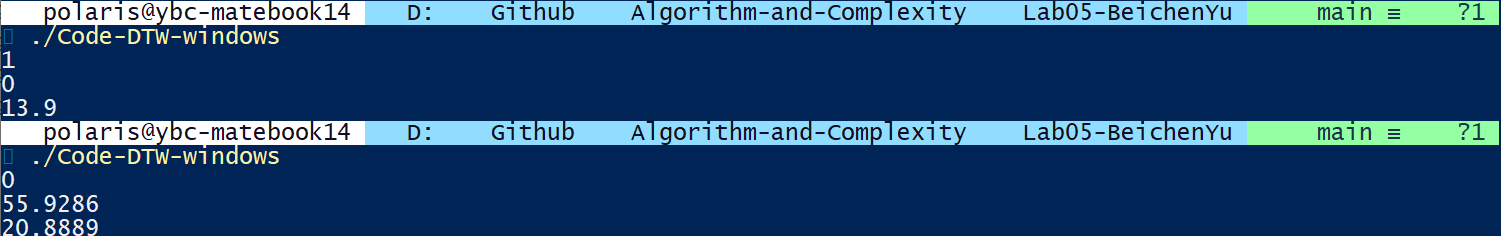
\includegraphics[width=0.8\textwidth]{dtw-w.png}
    \caption{The result of the DTW with constrain}
\end{figure}
		       \end{enumerate}
		    \end{solution}
		
	\end{enumerate}
	
	\vspace{20pt}
	
	\textbf{Remark:} You need to include your .pdf and .tex and {\color{red}\emph{$2$}} source code files in your uploaded .rar or .zip file. Screenshots of test case results are acceptable.
	
	%========================================================================
\end{document}
